\documentclass{standalone}
\usepackage{tikz}
\usetikzlibrary{patterns, positioning}


\begin{document}
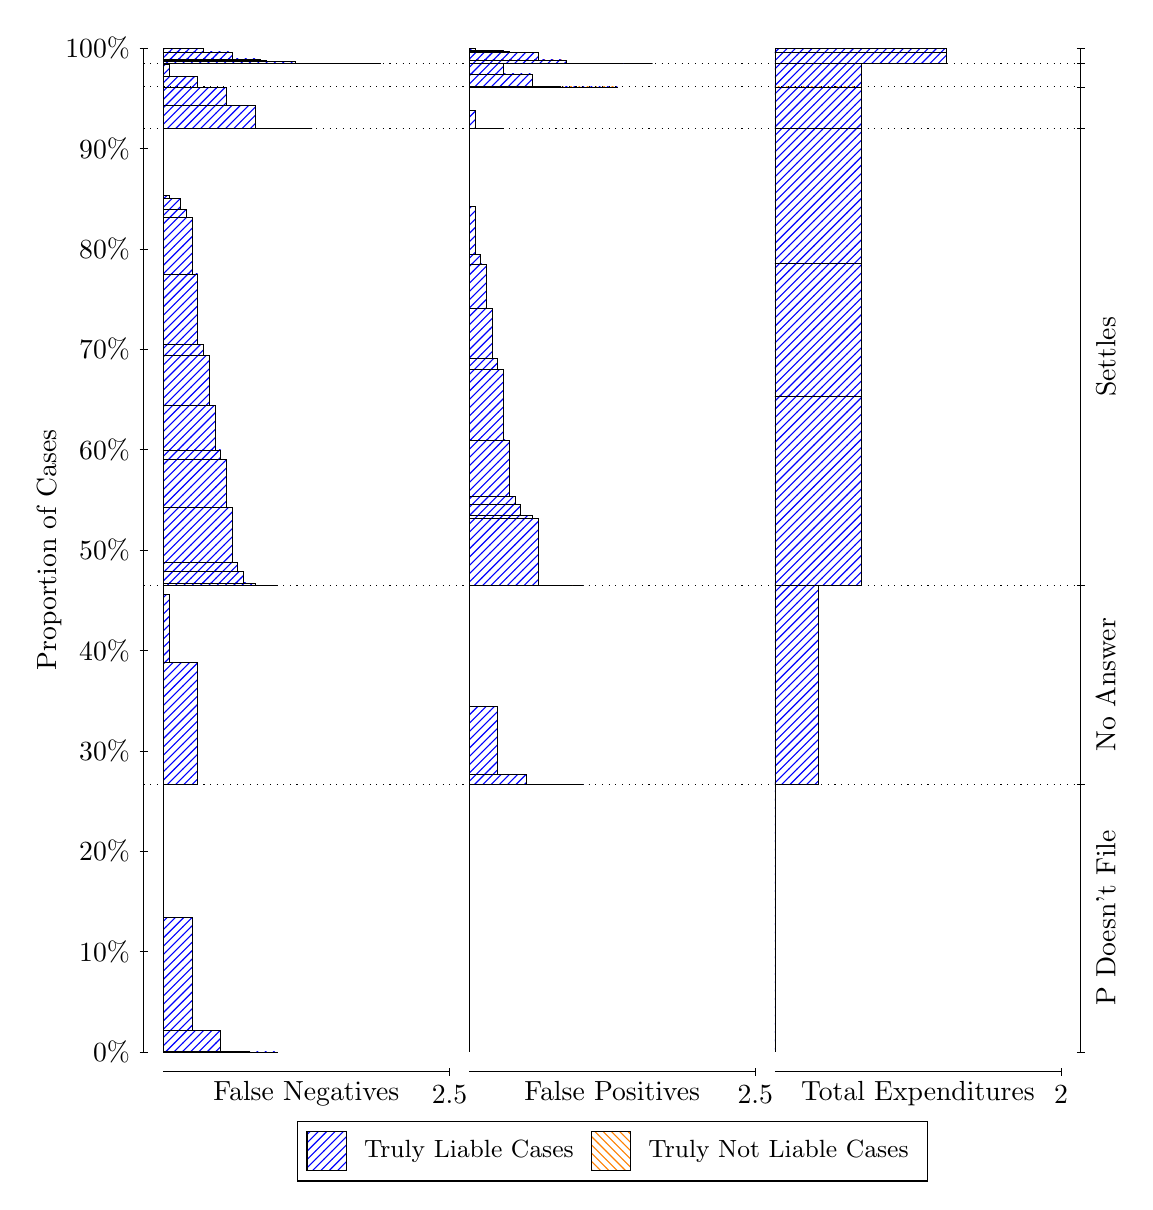
\begin{tikzpicture}
\draw[black, very thin] (1.5,1.75) -- (1.5,14.5);
\node[rotate=90, text=black, anchor=center] at (0.3, 8.125) {Proportion of Cases};
\draw[black, very thin] (1.45,1.75) -- (1.55,1.75);
\node[text=black, anchor=east] at (1.45, 1.75) {0\%};
\draw[black, very thin] (1.45,3.025) -- (1.55,3.025);
\node[text=black, anchor=east] at (1.45, 3.025) {10\%};
\draw[black, very thin] (1.45,4.3) -- (1.55,4.3);
\node[text=black, anchor=east] at (1.45, 4.3) {20\%};
\draw[black, very thin] (1.45,5.575) -- (1.55,5.575);
\node[text=black, anchor=east] at (1.45, 5.575) {30\%};
\draw[black, very thin] (1.45,6.85) -- (1.55,6.85);
\node[text=black, anchor=east] at (1.45, 6.85) {40\%};
\draw[black, very thin] (1.45,8.125) -- (1.55,8.125);
\node[text=black, anchor=east] at (1.45, 8.125) {50\%};
\draw[black, very thin] (1.45,9.4) -- (1.55,9.4);
\node[text=black, anchor=east] at (1.45, 9.4) {60\%};
\draw[black, very thin] (1.45,10.675) -- (1.55,10.675);
\node[text=black, anchor=east] at (1.45, 10.675) {70\%};
\draw[black, very thin] (1.45,11.95) -- (1.55,11.95);
\node[text=black, anchor=east] at (1.45, 11.95) {80\%};
\draw[black, very thin] (1.45,13.225) -- (1.55,13.225);
\node[text=black, anchor=east] at (1.45, 13.225) {90\%};
\draw[black, very thin] (1.45,14.5) -- (1.55,14.5);
\node[text=black, anchor=east] at (1.45, 14.5) {100\%};

\draw[black, very thin] (13.4,1.75) -- (13.4,14.5);
\draw[black, very thin] (13.35,1.75) -- (13.45,1.75);
\node[anchor=west] at (13.35, 1.75) {};
\draw[black, very thin] (13.35,5.1525) -- (13.45,5.1525);
\node[anchor=west] at (13.35, 5.1525) {};
\draw[black, very thin] (13.35,7.679) -- (13.45,7.679);
\node[anchor=west] at (13.35, 7.679) {};
\draw[black, very thin] (13.35,13.477) -- (13.45,13.477);
\node[anchor=west] at (13.35, 13.477) {};
\draw[black, very thin] (13.35,14.006) -- (13.45,14.006);
\node[anchor=west] at (13.35, 14.006) {};
\draw[black, very thin] (13.35,14.302) -- (13.45,14.302);
\node[anchor=west] at (13.35, 14.302) {};
\draw[black, very thin] (13.35,14.5) -- (13.45,14.5);
\node[anchor=west] at (13.35, 14.5) {};

\draw[black, very thin, pattern color=blue, pattern=north east lines] (1.75,1.75) rectangle (3.2033,1.75);
\draw[black, very thin, pattern color=blue, pattern=north east lines] (1.75,1.75) rectangle (2.84,1.7528);
\draw[black, very thin, pattern color=blue, pattern=north east lines] (1.75,1.7528) rectangle (2.4767,2.0248);
\draw[black, very thin, pattern color=blue, pattern=north east lines] (1.75,2.0248) rectangle (2.1133,3.4553);
\draw[black, very thin, pattern color=orange, pattern=north west lines] (1.75,3.4553) rectangle (1.75,3.4553);
\draw[black, very thin, pattern color=blue, pattern=north east lines] (1.75,3.4553) rectangle (1.75,5.1525);
\draw[black, very thin, pattern color=blue, pattern=north east lines] (1.75,5.1525) rectangle (2.186,6.6955);
\draw[black, very thin, pattern color=blue, pattern=north east lines] (1.75,6.6955) rectangle (1.8227,7.5603);
\draw[black, very thin, pattern color=orange, pattern=north west lines] (1.75,7.5603) rectangle (1.75,7.5603);
\draw[black, very thin, pattern color=blue, pattern=north east lines] (1.75,7.5603) rectangle (1.75,7.679);
\draw[black, very thin, pattern color=blue, pattern=north east lines] (1.75,7.679) rectangle (3.2033,7.679);
\draw[black, very thin, pattern color=blue, pattern=north east lines] (1.75,7.679) rectangle (3.058,7.6792);
\draw[black, very thin, pattern color=blue, pattern=north east lines] (1.75,7.6792) rectangle (2.9127,7.7055);
\draw[black, very thin, pattern color=blue, pattern=north east lines] (1.75,7.7055) rectangle (2.84,7.706);
\draw[black, very thin, pattern color=blue, pattern=north east lines] (1.75,7.706) rectangle (2.7673,7.8573);
\draw[black, very thin, pattern color=blue, pattern=north east lines] (1.75,7.8573) rectangle (2.6947,7.97);
\draw[black, very thin, pattern color=blue, pattern=north east lines] (1.75,7.97) rectangle (2.622,8.6672);
\draw[black, very thin, pattern color=blue, pattern=north east lines] (1.75,8.6672) rectangle (2.5493,9.2773);
\draw[black, very thin, pattern color=blue, pattern=north east lines] (1.75,9.2773) rectangle (2.4767,9.3975);
\draw[black, very thin, pattern color=blue, pattern=north east lines] (1.75,9.3975) rectangle (2.404,9.9664);
\draw[black, very thin, pattern color=blue, pattern=north east lines] (1.75,9.9664) rectangle (2.3313,10.598);
\draw[black, very thin, pattern color=blue, pattern=north east lines] (1.75,10.598) rectangle (2.2587,10.737);
\draw[black, very thin, pattern color=blue, pattern=north east lines] (1.75,10.737) rectangle (2.186,11.631);
\draw[black, very thin, pattern color=blue, pattern=north east lines] (1.75,11.631) rectangle (2.1133,12.346);
\draw[black, very thin, pattern color=blue, pattern=north east lines] (1.75,12.346) rectangle (2.0407,12.454);
\draw[black, very thin, pattern color=blue, pattern=north east lines] (1.75,12.454) rectangle (1.968,12.59);
\draw[black, very thin, pattern color=blue, pattern=north east lines] (1.75,12.59) rectangle (1.8953,12.592);
\draw[black, very thin, pattern color=blue, pattern=north east lines] (1.75,12.592) rectangle (1.8227,12.627);
\draw[black, very thin, pattern color=orange, pattern=north west lines] (1.75,12.627) rectangle (1.75,12.627);
\draw[black, very thin, pattern color=blue, pattern=north east lines] (1.75,12.627) rectangle (1.75,13.477);
\draw[black, very thin, pattern color=blue, pattern=north east lines] (1.75,13.477) rectangle (3.6393,13.477);
\draw[black, very thin, pattern color=blue, pattern=north east lines] (1.75,13.477) rectangle (3.276,13.483);
\draw[black, very thin, pattern color=blue, pattern=north east lines] (1.75,13.483) rectangle (2.9127,13.774);
\draw[black, very thin, pattern color=blue, pattern=north east lines] (1.75,13.774) rectangle (2.5493,14.003);
\draw[black, very thin, pattern color=blue, pattern=north east lines] (1.75,14.003) rectangle (2.186,14.006);
\draw[black, very thin, pattern color=orange, pattern=north west lines] (1.75,14.006) rectangle (1.75,14.006);
\draw[black, very thin, pattern color=blue, pattern=north east lines] (1.75,14.006) rectangle (2.186,14.136);
\draw[black, very thin, pattern color=blue, pattern=north east lines] (1.75,14.136) rectangle (1.8227,14.294);
\draw[black, very thin, pattern color=orange, pattern=north west lines] (1.75,14.294) rectangle (1.75,14.294);
\draw[black, very thin, pattern color=blue, pattern=north east lines] (1.75,14.294) rectangle (1.75,14.302);
\draw[black, very thin, pattern color=blue, pattern=north east lines] (1.75,14.302) rectangle (4.5113,14.302);
\draw[black, very thin, pattern color=blue, pattern=north east lines] (1.75,14.302) rectangle (4.148,14.302);
\draw[black, very thin, pattern color=blue, pattern=north east lines] (1.75,14.302) rectangle (3.7847,14.306);
\draw[black, very thin, pattern color=blue, pattern=north east lines] (1.75,14.306) rectangle (3.712,14.306);
\draw[black, very thin, pattern color=blue, pattern=north east lines] (1.75,14.306) rectangle (3.4213,14.334);
\draw[black, very thin, pattern color=blue, pattern=north east lines] (1.75,14.334) rectangle (3.3487,14.334);
\draw[black, very thin, pattern color=blue, pattern=north east lines] (1.75,14.334) rectangle (3.058,14.343);
\draw[black, very thin, pattern color=blue, pattern=north east lines] (1.75,14.343) rectangle (2.9853,14.361);
\draw[black, very thin, pattern color=blue, pattern=north east lines] (1.75,14.361) rectangle (2.6947,14.361);
\draw[black, very thin, pattern color=blue, pattern=north east lines] (1.75,14.361) rectangle (2.622,14.452);
\draw[black, very thin, pattern color=blue, pattern=north east lines] (1.75,14.452) rectangle (2.3313,14.452);
\draw[black, very thin, pattern color=blue, pattern=north east lines] (1.75,14.452) rectangle (2.2587,14.498);
\draw[black, very thin, pattern color=blue, pattern=north east lines] (1.75,14.498) rectangle (1.8953,14.5);
\draw[black, very thin, pattern color=orange, pattern=north west lines] (1.75,14.5) rectangle (1.75,14.5);
\draw[black, very thin, pattern color=blue, pattern=north east lines] (1.75,14.5) rectangle (1.75,14.5);
\draw[black, very thin, pattern color=orange, pattern=north west lines] (5.6333,1.75) rectangle (5.6333,1.75);
\draw[black, very thin, pattern color=blue, pattern=north east lines] (5.6333,1.75) rectangle (5.6333,5.1525);
\draw[black, very thin, pattern color=orange, pattern=north west lines] (5.6333,5.1525) rectangle (7.0867,5.1525);
\draw[black, very thin, pattern color=blue, pattern=north east lines] (5.6333,5.1525) rectangle (7.0867,5.1525);
\draw[black, very thin, pattern color=blue, pattern=north east lines] (5.6333,5.1525) rectangle (6.7233,5.1528);
\draw[black, very thin, pattern color=blue, pattern=north east lines] (5.6333,5.1528) rectangle (6.36,5.2713);
\draw[black, very thin, pattern color=blue, pattern=north east lines] (5.6333,5.2713) rectangle (5.9967,6.136);
\draw[black, very thin, pattern color=blue, pattern=north east lines] (5.6333,6.136) rectangle (5.6333,7.679);
\draw[black, very thin, pattern color=orange, pattern=north west lines] (5.6333,7.679) rectangle (7.0867,7.679);
\draw[black, very thin, pattern color=blue, pattern=north east lines] (5.6333,7.679) rectangle (7.0867,7.679);
\draw[black, very thin, pattern color=orange, pattern=north west lines] (5.6333,7.679) rectangle (6.9413,7.679);
\draw[black, very thin, pattern color=blue, pattern=north east lines] (5.6333,7.679) rectangle (6.9413,7.679);
\draw[black, very thin, pattern color=orange, pattern=north west lines] (5.6333,7.679) rectangle (6.796,7.679);
\draw[black, very thin, pattern color=blue, pattern=north east lines] (5.6333,7.679) rectangle (6.796,7.679);
\draw[black, very thin, pattern color=blue, pattern=north east lines] (5.6333,7.679) rectangle (6.7233,7.679);
\draw[black, very thin, pattern color=orange, pattern=north west lines] (5.6333,7.679) rectangle (6.6507,7.679);
\draw[black, very thin, pattern color=blue, pattern=north east lines] (5.6333,7.679) rectangle (6.6507,7.6803);
\draw[black, very thin, pattern color=blue, pattern=north east lines] (5.6333,7.6803) rectangle (6.578,7.6805);
\draw[black, very thin, pattern color=orange, pattern=north west lines] (5.6333,7.6805) rectangle (6.5053,7.6805);
\draw[black, very thin, pattern color=blue, pattern=north east lines] (5.6333,7.6805) rectangle (6.5053,8.5292);
\draw[black, very thin, pattern color=blue, pattern=north east lines] (5.6333,8.5292) rectangle (6.4327,8.5638);
\draw[black, very thin, pattern color=blue, pattern=north east lines] (5.6333,8.5638) rectangle (6.36,8.5652);
\draw[black, very thin, pattern color=blue, pattern=north east lines] (5.6333,8.5652) rectangle (6.2873,8.7018);
\draw[black, very thin, pattern color=blue, pattern=north east lines] (5.6333,8.7018) rectangle (6.2147,8.8092);
\draw[black, very thin, pattern color=blue, pattern=north east lines] (5.6333,8.8092) rectangle (6.142,9.5245);
\draw[black, very thin, pattern color=blue, pattern=north east lines] (5.6333,9.5245) rectangle (6.0693,10.418);
\draw[black, very thin, pattern color=blue, pattern=north east lines] (5.6333,10.418) rectangle (5.9967,10.558);
\draw[black, very thin, pattern color=blue, pattern=north east lines] (5.6333,10.558) rectangle (5.924,11.189);
\draw[black, very thin, pattern color=blue, pattern=north east lines] (5.6333,11.189) rectangle (5.8513,11.758);
\draw[black, very thin, pattern color=blue, pattern=north east lines] (5.6333,11.758) rectangle (5.7787,11.878);
\draw[black, very thin, pattern color=blue, pattern=north east lines] (5.6333,11.878) rectangle (5.706,12.488);
\draw[black, very thin, pattern color=blue, pattern=north east lines] (5.6333,12.488) rectangle (5.6333,13.477);
\draw[black, very thin, pattern color=orange, pattern=north west lines] (5.6333,13.477) rectangle (6.0693,13.477);
\draw[black, very thin, pattern color=blue, pattern=north east lines] (5.6333,13.477) rectangle (6.0693,13.479);
\draw[black, very thin, pattern color=blue, pattern=north east lines] (5.6333,13.479) rectangle (5.706,13.709);
\draw[black, very thin, pattern color=blue, pattern=north east lines] (5.6333,13.709) rectangle (5.6333,14.006);
\draw[black, very thin, pattern color=orange, pattern=north west lines] (5.6333,14.006) rectangle (7.5227,14.006);
\draw[black, very thin, pattern color=blue, pattern=north east lines] (5.6333,14.006) rectangle (7.5227,14.006);
\draw[black, very thin, pattern color=blue, pattern=north east lines] (5.6333,14.006) rectangle (7.1593,14.006);
\draw[black, very thin, pattern color=blue, pattern=north east lines] (5.6333,14.006) rectangle (6.796,14.014);
\draw[black, very thin, pattern color=blue, pattern=north east lines] (5.6333,14.014) rectangle (6.4327,14.172);
\draw[black, very thin, pattern color=blue, pattern=north east lines] (5.6333,14.172) rectangle (6.0693,14.302);
\draw[black, very thin, pattern color=orange, pattern=north west lines] (5.6333,14.302) rectangle (7.9587,14.302);
\draw[black, very thin, pattern color=blue, pattern=north east lines] (5.6333,14.302) rectangle (7.9587,14.302);
\draw[black, very thin, pattern color=orange, pattern=north west lines] (5.6333,14.302) rectangle (7.5953,14.302);
\draw[black, very thin, pattern color=blue, pattern=north east lines] (5.6333,14.302) rectangle (7.5953,14.302);
\draw[black, very thin, pattern color=orange, pattern=north west lines] (5.6333,14.302) rectangle (7.232,14.302);
\draw[black, very thin, pattern color=blue, pattern=north east lines] (5.6333,14.302) rectangle (7.232,14.304);
\draw[black, very thin, pattern color=blue, pattern=north east lines] (5.6333,14.304) rectangle (6.8687,14.35);
\draw[black, very thin, pattern color=orange, pattern=north west lines] (5.6333,14.35) rectangle (6.8687,14.35);
\draw[black, very thin, pattern color=blue, pattern=north east lines] (5.6333,14.35) rectangle (6.8687,14.35);
\draw[black, very thin, pattern color=orange, pattern=north west lines] (5.6333,14.35) rectangle (6.796,14.35);
\draw[black, very thin, pattern color=blue, pattern=north east lines] (5.6333,14.35) rectangle (6.796,14.35);
\draw[black, very thin, pattern color=blue, pattern=north east lines] (5.6333,14.35) rectangle (6.5053,14.44);
\draw[black, very thin, pattern color=blue, pattern=north east lines] (5.6333,14.44) rectangle (6.5053,14.441);
\draw[black, very thin, pattern color=orange, pattern=north west lines] (5.6333,14.441) rectangle (6.4327,14.441);
\draw[black, very thin, pattern color=blue, pattern=north east lines] (5.6333,14.441) rectangle (6.4327,14.441);
\draw[black, very thin, pattern color=blue, pattern=north east lines] (5.6333,14.441) rectangle (6.142,14.45);
\draw[black, very thin, pattern color=blue, pattern=north east lines] (5.6333,14.45) rectangle (6.142,14.459);
\draw[black, very thin, pattern color=blue, pattern=north east lines] (5.6333,14.459) rectangle (6.0693,14.467);
\draw[black, very thin, pattern color=orange, pattern=north west lines] (5.6333,14.467) rectangle (6.0693,14.467);
\draw[black, very thin, pattern color=blue, pattern=north east lines] (5.6333,14.467) rectangle (6.0693,14.467);
\draw[black, very thin, pattern color=blue, pattern=north east lines] (5.6333,14.467) rectangle (5.7787,14.467);
\draw[black, very thin, pattern color=blue, pattern=north east lines] (5.6333,14.467) rectangle (5.7787,14.467);
\draw[black, very thin, pattern color=blue, pattern=north east lines] (5.6333,14.467) rectangle (5.706,14.495);
\draw[black, very thin, pattern color=blue, pattern=north east lines] (5.6333,14.495) rectangle (5.706,14.496);
\draw[black, very thin, pattern color=blue, pattern=north east lines] (5.6333,14.496) rectangle (5.6333,14.5);
\draw[black, very thin, pattern color=orange, pattern=north west lines] (9.5167,1.75) rectangle (9.5167,1.75);
\draw[black, very thin, pattern color=blue, pattern=north east lines] (9.5167,1.75) rectangle (9.5167,5.1525);
\draw[black, very thin, pattern color=orange, pattern=north west lines] (9.5167,5.1525) rectangle (10.062,5.1525);
\draw[black, very thin, pattern color=blue, pattern=north east lines] (9.5167,5.1525) rectangle (10.062,7.679);
\draw[black, very thin, pattern color=orange, pattern=north west lines] (9.5167,7.679) rectangle (10.607,7.679);
\draw[black, very thin, pattern color=blue, pattern=north east lines] (9.5167,7.679) rectangle (10.607,10.082);
\draw[black, very thin, pattern color=orange, pattern=north west lines] (9.5167,10.082) rectangle (10.607,10.082);
\draw[black, very thin, pattern color=blue, pattern=north east lines] (9.5167,10.082) rectangle (10.607,11.766);
\draw[black, very thin, pattern color=orange, pattern=north west lines] (9.5167,11.766) rectangle (10.607,11.766);
\draw[black, very thin, pattern color=blue, pattern=north east lines] (9.5167,11.766) rectangle (10.607,13.477);
\draw[black, very thin, pattern color=orange, pattern=north west lines] (9.5167,13.477) rectangle (10.607,13.477);
\draw[black, very thin, pattern color=blue, pattern=north east lines] (9.5167,13.477) rectangle (10.607,14.006);
\draw[black, very thin, pattern color=orange, pattern=north west lines] (9.5167,14.006) rectangle (10.607,14.006);
\draw[black, very thin, pattern color=blue, pattern=north east lines] (9.5167,14.006) rectangle (10.607,14.302);
\draw[black, very thin, pattern color=orange, pattern=north west lines] (9.5167,14.302) rectangle (11.697,14.302);
\draw[black, very thin, pattern color=blue, pattern=north east lines] (9.5167,14.302) rectangle (11.697,14.449);
\draw[black, very thin, pattern color=orange, pattern=north west lines] (9.5167,14.449) rectangle (11.697,14.449);
\draw[black, very thin, pattern color=blue, pattern=north east lines] (9.5167,14.449) rectangle (11.697,14.5);
\draw[black, dotted] (1.5,5.1525) -- (13.4,5.1525);
\draw[black, dotted] (1.5,7.679) -- (13.4,7.679);
\draw[black, dotted] (1.5,13.477) -- (13.4,13.477);
\draw[black, dotted] (1.5,14.006) -- (13.4,14.006);
\draw[black, dotted] (1.5,14.302) -- (13.4,14.302);
\draw[black, very thin] (1.75,1.5) -- (5.3833,1.5);
\node[text=black, anchor=north] at (3.5667, 1.5) {False Negatives};
\draw[black, very thin] (5.3833,1.45) -- (5.3833,1.55);
\node[text=black, anchor=north] at (5.3833, 1.45) {2.5};

\draw[black, very thin] (5.6333,1.5) -- (9.2667,1.5);
\node[text=black, anchor=north] at (7.45, 1.5) {False Positives};
\draw[black, very thin] (9.2667,1.45) -- (9.2667,1.55);
\node[text=black, anchor=north] at (9.2667, 1.45) {2.5};

\draw[black, very thin] (9.5167,1.5) -- (13.15,1.5);
\node[text=black, anchor=north] at (11.333, 1.5) {Total Expenditures};
\draw[black, very thin] (13.15,1.45) -- (13.15,1.55);
\node[text=black, anchor=north] at (13.15, 1.45) {2};

\node[text=black, centered, rotate=90] at (13.72, 3.4513) {P Doesn't File};
\node[text=black, centered, rotate=90] at (13.72, 6.4158) {No Answer};
\node[text=black, centered, rotate=90] at (13.72, 10.578) {Settles};




\draw (7.449999999999999,1.5) node[draw=none] (baseCoordinate) {};
\begin{scope}[align=center]
        \matrix[scale=0.5, draw=black, below=0.5cm of baseCoordinate, nodes={draw}, column sep=0.1cm]{
            \node[rectangle, draw, minimum width=0.5cm, minimum height=0.5cm, pattern color=blue, pattern=north east lines] {}; &
            \node[draw=none, font=\small, text=black] (B) {Truly Liable Cases}; &
            \node[rectangle, draw, minimum width=0.5cm, minimum height=0.5cm, pattern color=orange, pattern=north west lines] {}; &
            \node[draw=none, font=\small, text=black] (B) {Truly Not Liable Cases}; \\
            };
\end{scope}

\end{tikzpicture}
\end{document}